\documentclass{article}
\usepackage{122}

\usepackage{array}
\usepackage{graphicx}
\usepackage[hidelinks,bookmarks=false]{hyperref}
\usepackage{attachfile2}

\title{Биоинформатика \\ Домашнее задание №3}

\graphicspath{ {../bio/sars2/screenshots/} }
\newcolumntype{C}{ >{\centering\arraybackslash} m{.3\textwidth} }

\begin{document}
  \maketitle

  \section{Скачанные коронавирусы}
  \begin{center}
    \begin{tabular}{|c|l|l|l|l|l|}
      \hline
      № & Подвид & Страна & Дата & ссылка на NCBI & файл
      \\\hline
      1 & SARS-CoV-2 & Japan & 2020-03 & \href{https://www.ncbi.nlm.nih.gov/nuccore/LC581364}{\texttt{LC581364}} & \attachfile{../bio/sars2/fasta/LC581364.fasta} \\
      2 & SARS-CoV-2 & South & 2020-03-07 & \href{https://www.ncbi.nlm.nih.gov/nuccore/MT324062}{\texttt{MT324062}} & \attachfile{../bio/sars2/fasta/MT324062.fasta} \\
      3 & SARS-CoV-2 & Italy & 2020-02-26 & \href{https://www.ncbi.nlm.nih.gov/nuccore/MT479216}{\texttt{MT479216}} & \attachfile{../bio/sars2/fasta/MT479216.fasta} \\
      4 & SARS-CoV-2 & Netherlands & 2020-03-03 & \href{https://www.ncbi.nlm.nih.gov/nuccore/MT705205}{\texttt{MT705205}} & \attachfile{../bio/sars2/fasta/MT705205.fasta} \\
      5 & SARS-CoV-2 & New Zealand & 2020-03-21 & \href{https://www.ncbi.nlm.nih.gov/nuccore/MT706050}{\texttt{MT706050}} & \attachfile{../bio/sars2/fasta/MT706050.fasta} \\
      6 & SARS-CoV-2 & Russia & 2020-04-17 & \href{https://www.ncbi.nlm.nih.gov/nuccore/MT890462}{\texttt{MT890462}} & \attachfile{../bio/sars2/fasta/MT890462.fasta} \\
      7 & SARS-CoV-2 & Egypt & 2020-09-29 & \href{https://www.ncbi.nlm.nih.gov/nuccore/MW250352}{\texttt{MW250352}} & \attachfile{../bio/sars2/fasta/MW250352.fasta} \\
      8 & SARS-CoV-2 & Romania & 2020-07-20 & \href{https://www.ncbi.nlm.nih.gov/nuccore/MW255830}{\texttt{MW255830}} & \attachfile{../bio/sars2/fasta/MW255830.fasta} \\
      9 & SARS-CoV-1 & Canada (RefSeq) & 2003 & \href{https://www.ncbi.nlm.nih.gov/nuccore/NC_004718}{\texttt{NC\_004718}} & \attachfile{../bio/sars2/fasta/NC_004718.fasta} \\
      10 & SARS-CoV-2 & China (RefSeq) & 2019-12 & \href{https://www.ncbi.nlm.nih.gov/nuccore/NC_045512}{\texttt{NC\_045512}} & \attachfile{../bio/sars2/fasta/NC_045512.fasta} \\
      \hline
    \end{tabular}
  \end{center}

  \section{Выравнивание}
  Тут MEGA совсем не справилась с выравниванием таких длинных последовательностей,
  и поэтому пришлось воспользоватся \href{http://www.clustal.org/omega/}{Clustal Omega}. \\
  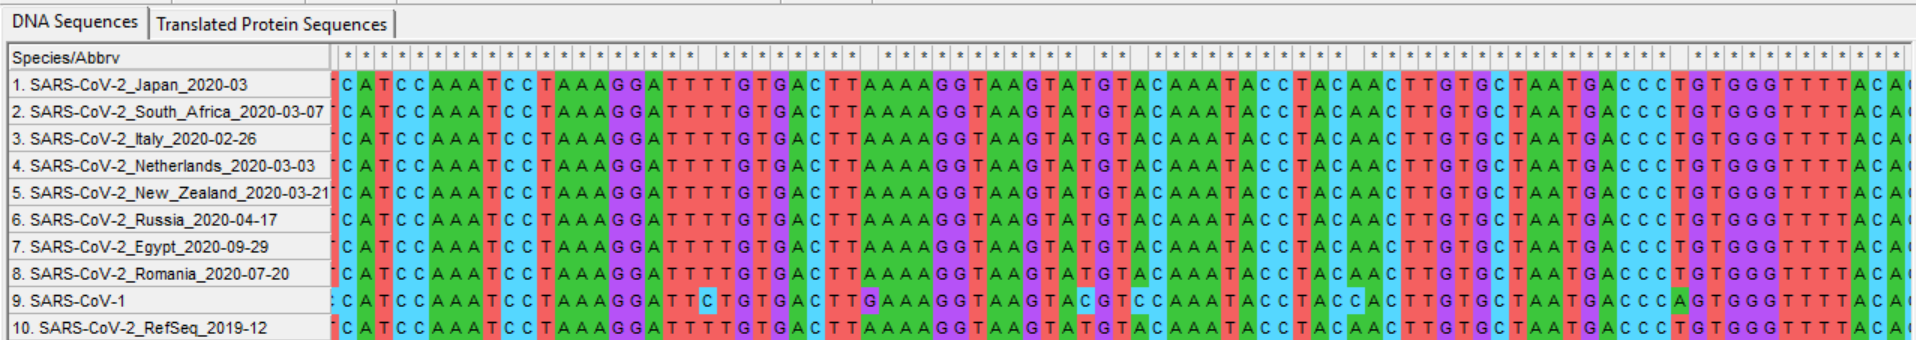
\includegraphics[width=\textwidth]{aligned.png}

  \section{Деревья}
  Нам зачем-то надо нарисовать 3 дерева, хотя мне кажется они все получились норм (дальше используется третье).
  \begin{center}
    \begin{tabular}{|C|C|C|}
      \hline
      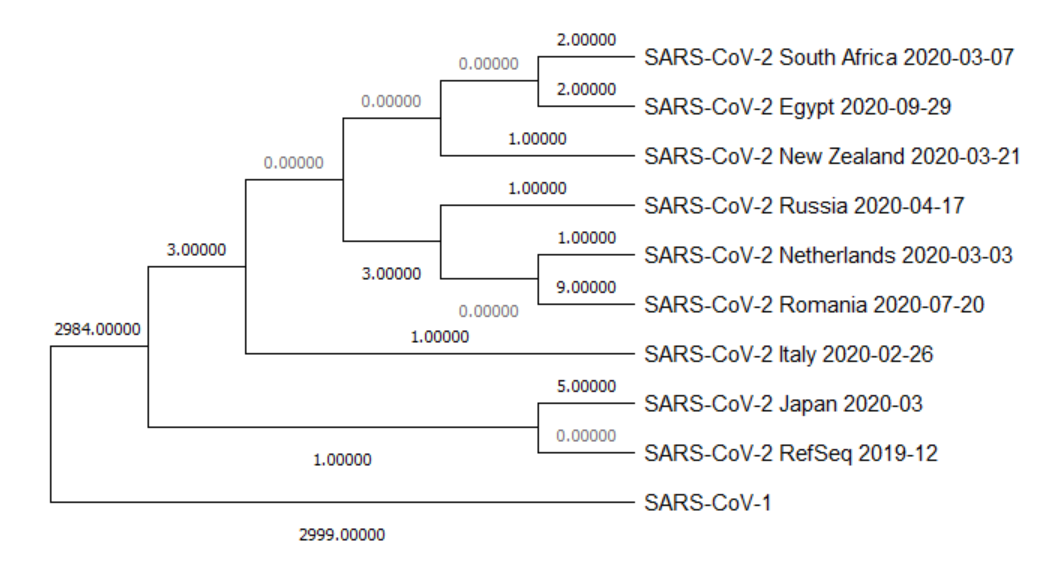
\includegraphics[width=.3\textwidth]{treeMP.png} &
      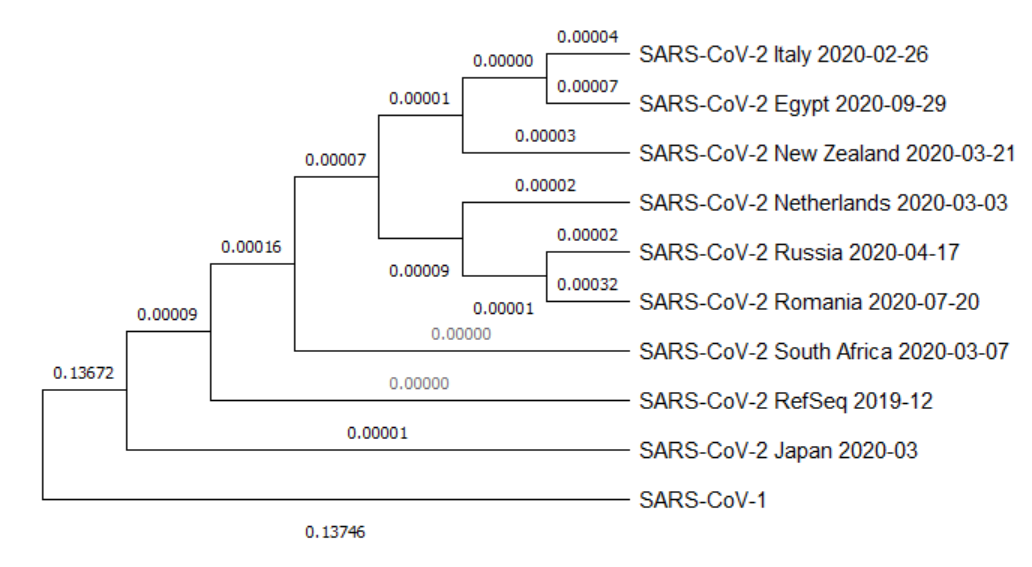
\includegraphics[width=.3\textwidth]{treeNJ.png} &
      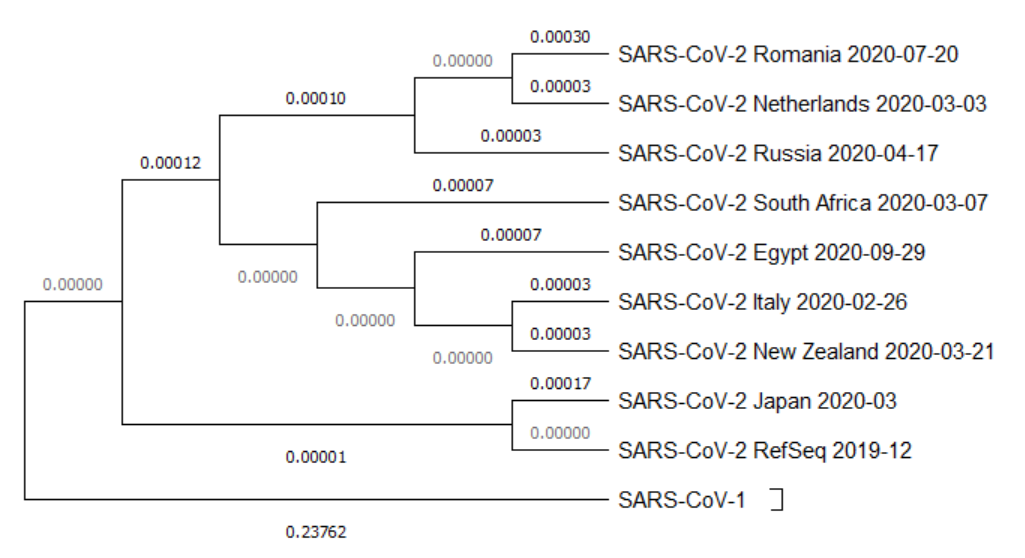
\includegraphics[width=.3\textwidth]{fulltree.png} \\\hline
      Maximum Parsimony &
      Neighbor Joining &
      Maximum Likelihood \\\hline
    \end{tabular}
  \end{center}

  \section{Дерево}
  Тут сначала дерево получилось с очень маленькими длинами веток,
  и чтобы сравнить пришлось отдельно нарисовать поддерево для SARS-CoV-2.
  У нас получилось что RefSeq и Romania самый близкий и далёкий от SARS-CoV-1, и поэтому на мутации мы будем проверять именно их.
  Также по этому дереву видно что вирус первый заразил Китай, а последний Румынию (хотя дата на вирусе из Египта стоит позже). \\
  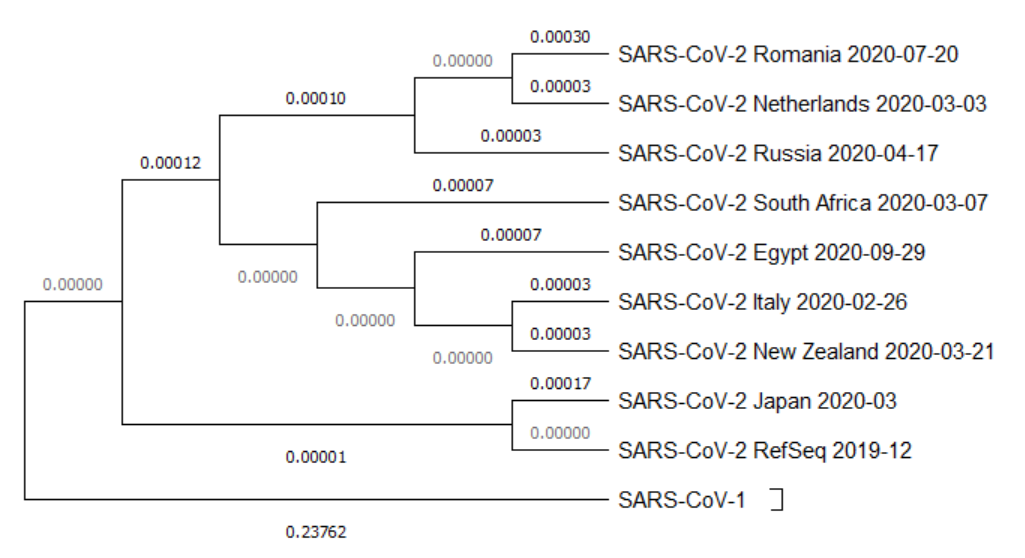
\includegraphics[width=.5\textwidth]{fulltree.png}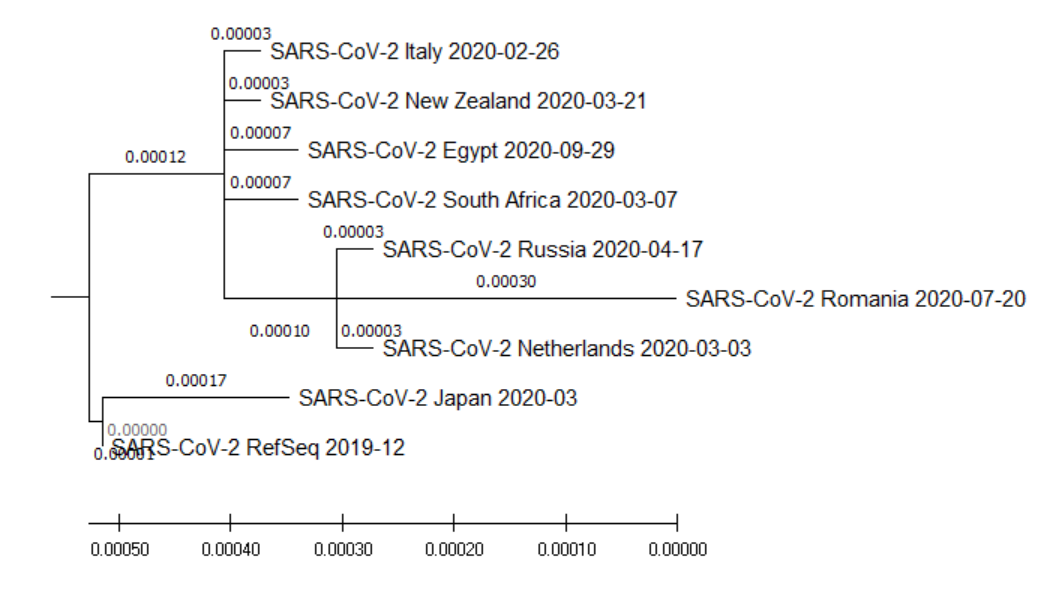
\includegraphics[width=.5\textwidth]{deeptree.png}

  \section{Скриншоты мутаций}
  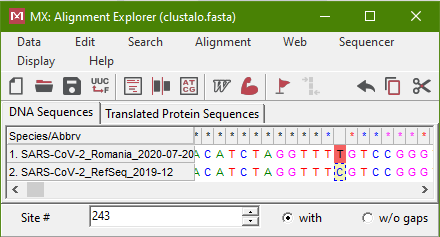
\includegraphics[width=.33\textwidth]{mutation1.png}
  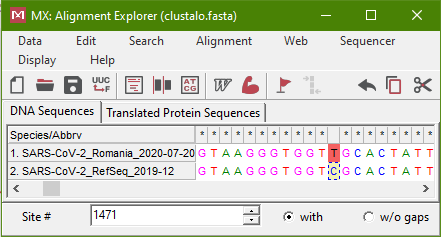
\includegraphics[width=.33\textwidth]{mutation2.png}
  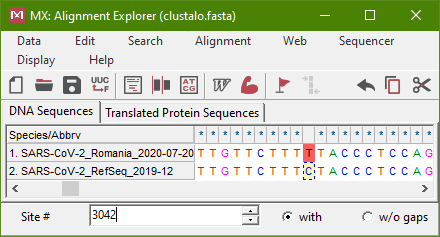
\includegraphics[width=.33\textwidth]{mutation3.png} \\
  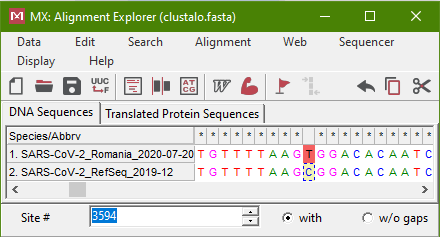
\includegraphics[width=.33\textwidth]{mutation4.png}
  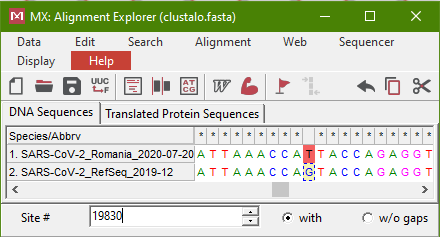
\includegraphics[width=.33\textwidth]{mutation5.png}
  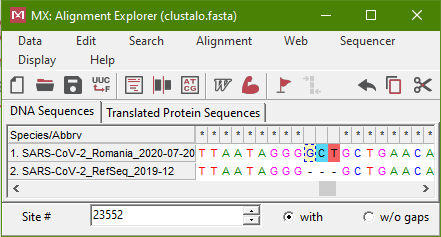
\includegraphics[width=.33\textwidth]{mutation6.png} \\
  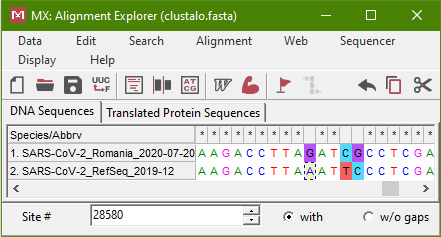
\includegraphics[width=.33\textwidth]{mutation7.png}
  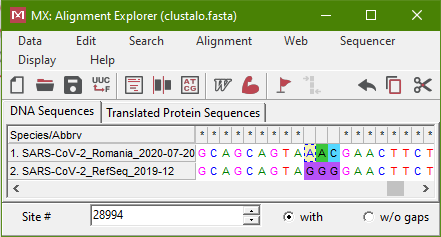
\includegraphics[width=.33\textwidth]{mutation8.png}
  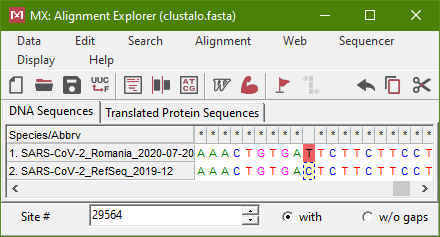
\includegraphics[width=.33\textwidth]{mutation9.png}

  \section{Список мутаций}
  \begin{center}
    \begin{tabular}{|c|l|l|}
      \hline
      № & Координаты & Попадание
      \\\hline
      1 & 143 & до первого гена \\
      2 & 1471 & orf1a polyprotein и orf1ab polyprotein \\
      3 & 3042 & orf1a polyprotein и orf1ab polyprotein \\
      4 & 3594 & orf1a polyprotein и orf1ab polyprotein \\
      5 & 19830 & orf1ab polyprotein \\
      6 & 23552 & surface glycoprotein \\
      7 & 28580 & nucleocapsid phosphoprotein \\
      8 & 28994 & nucleocapsid phosphoprotein \\
      9 & 29564 & ORF10 protein \\
      \hline
    \end{tabular}
  \end{center}

\end{document}
